\documentclass[12pt,chapterheads]{ucsd}

\usepackage[paper=letterpaper]{geometry}
\usepackage{amsmath, amscd, amssymb, amsthm}
\usepackage{graphicx}
\usepackage[T1]{fontenc}
\usepackage{makeidx}
\usepackage{boxedminipage}
\usepackage{setspace}
\usepackage{url}
\usepackage{balance}
\usepackage{color}
\usepackage{textcomp}
\usepackage{booktabs}
\usepackage{ccicons}
\usepackage{comment}
\usepackage{wrapfig}
\usepackage{tabulary}
\usepackage{float}
\usepackage[colorlinks=true, 
            pdfstartview=FitV, 
            linkcolor=black, 
            citecolor=black, 
            urlcolor=black,
            plainpages=false,
            pdfpagelabels]{hyperref}

\hypersetup{ 
    pdfauthor = {Your Name Here}, 
    pdftitle = {The Title of The Dissertation}, 
    pdfkeywords = {Keywords for Searching}, 
    pdfcreator = {pdfLaTeX with hyperref package}, 
    pdfproducer = {pdfLaTeX}}

\newenvironment{mynote}{
    \medskip
    \noindent
    \let\emph=\textbf
    \begin{boxedminipage}{\columnwidth}
}{
    \end{boxedminipage}\vspace{0.5em}
}

\newcommand{\rev}[1]{#1}

\def\fig#1{Figure~\ref{#1}}
\def\tab#1{Table~\ref{#1}}
\def\eqn#1{Equation~\ref{#1}}

\hyphenation{ana-ly-sis}
\hyphenation{ana-ly-ses}
\hyphenation{app-li-ca-tions}
\hyphenation{macOS}
\hyphenation{Deja-View}
\hyphenation{Demo-Wiz}
\hyphenation{Power-Point}
\hyphenation{Apple-Script}
\hyphenation{FFmpeg}
\hyphenation{Cour-sera}
\hyphenation{bi-directional}
\hyphenation{MATLAB}
\hyphenation{ubi-qui-tous}
\hyphenation{LaTeX}
\hyphenation{tool-kits}

\makeindex

\begin{document}

\hyphenation{ana-ly-sis}
\hyphenation{ana-ly-ses}
\hyphenation{app-li-ca-tions}
\hyphenation{macOS}
\hyphenation{Deja-View}
\hyphenation{Demo-Wiz}
\hyphenation{Power-Point}
\hyphenation{Apple-Script}
\hyphenation{FFmpeg}
\makeindex

\begin{document}

\title{Operating System monitoring for programming tutorial creation and evaluation}
\author{Alok Shankar Mysore}
\degreeyear{2018}
\degree{Masters} 
\field{Computer Science}
\chair{Professor Philip J. Guo}
\othermembers{
Professor Scott R. Klemmer\\ 
Professor Leo Porter\\
}
\numberofmembers{3}

\begin{frontmatter}
\makefrontmatter
%% DEDICATION
% You have three choices here:
%   1. Use the ``dedication'' environment.   Put in the text you want,
%   and you'll get a perfectly respectable dedication page.
%
%   2. Use the ``mydedication'' environment.  If you don't like the
%   formatting of option 1, use this environment and format things
%   however you wish.
%
%   3. If you don't want a dedication, it's not required.

\begin{dedication} % The style file will format this for you.
  lol idk
\end{dedication}
% \begin{epigraph} % The style file will position the text for you.
%   \emph{A careful quotation\\
%   conveys brilliance.}\\
%   ---Smarty Pants
% \end{epigraph}
%% ACKNOWLEDGEMENTS
%  While technically optional, you probably have someone to thank.
%  Also, a paragraph acknowledging all coauthors and publishers (if
%  you have any) is required in the acknowledgements page and as the
%  last paragraph of text at the end of each respective chapter. See
%  the OGS Formatting Manual for more information.

\begin{acknowledgements} 
People to thank:
  	1. Philip
    2. Scott
\end{acknowledgements}
%% VITA
%  A brief vita is required in a doctoral thesis. See the OGS
%  Formatting Manual for more information.

\begin{vitapage}
\begin{vita}
  \item[2002] B.~S. in Mathematics \emph{cum laude}, University of Southern North Dakota, Hoople
  \item[2002-2007] Graduate Teaching Assistant, University of California, San Diego
  \item[2007] Ph.~D. in Mathematics, University of California, San Diego 
\end{vita}
\begin{publications}
  \item Your Name, ``A Simple Proof Of The Riemann Hypothesis'', \emph{Annals of Math}, 314, 2007.
  \item Your Name, Euclid, ``There Are Lots Of Prime Numbers'', \emph{Journal of Primes}, 1, 300
	B.C.
\end{publications}
\end{vitapage}
\begin{abstract}
Lorem ipsum dolor sit amet, consectetur adipiscing elit. Vivamus et erat dolor. Proin posuere aliquam libero. Integer tellus diam, tempus lobortis tortor eget, hendrerit tempor sapien. Praesent ut laoreet arcu. Mauris eget varius turpis. Praesent venenatis sapien in risus rutrum, id mattis felis rutrum. Vestibulum tincidunt luctus dui, sed malesuada sem dictum in. Sed id enim suscipit magna ultricies suscipit. Maecenas placerat at mauris ut feugiat. Proin lacinia feugiat pharetra. Orci varius natoque penatibus et magnis dis parturient montes, nascetur ridiculus mus. Vestibulum quis sollicitudin est, nec luctus arcu.

Vestibulum a odio mi. Cras facilisis felis vel enim interdum blandit. Mauris porttitor nisl ipsum, eget rhoncus felis tempus eu. Mauris pellentesque tincidunt nulla nec pretium. Vestibulum accumsan convallis ante at feugiat. Fusce placerat lorem eros, eget feugiat metus dictum quis. Vestibulum suscipit nulla justo, at feugiat lacus ultricies sed. In hac habitasse platea dictumst. In eleifend mauris at metus sollicitudin, quis dictum purus efficitur. Ut interdum dolor ac neque lobortis accumsan.

Sed varius varius sapien eu fermentum. Donec vestibulum vel ipsum id finibus. Ut consequat tempor dapibus. Ut tristique lectus magna, scelerisque bibendum libero mollis vel. Maecenas luctus elit ac aliquam egestas. Mauris consectetur blandit libero, in tincidunt ante fermentum.
\end{abstract}
\end{frontmatter}

\chapter{Introduction}
It can be hard for experts in any field to write high-quality
documentation, instructional materials, and step-by-step tutorials. Instructional materials such as these are vital for helping people such as
software developers, data scientists, researchers, and system
administrators perform complex software-based tasks. 

One can either create a written tutorial by painstakingly enumerating 
all steps, describing shell commands, expected outputs, and side-effects,
and taking screenshots to illustrate GUI actions. Or one can demonstrate
all of the steps and record a screencast video, but it is tedious
to later fix bugs in videos. Neither approach is ideal for
creators. Also, neither is ideal for people trying to follow these
tutorials: manually-written tutorials may skip over critical details
~\cite{Lafreniere2013}, and videos can be difficult to browse and
navigate~\cite{Krosnick2014,Pavel2014}.

Additionally, once these tutorials are created, their creators cannot
easily get a sense of how people navigate through them or what parts 
they frequently get stuck on. They also cannot easily predict where 
new users might struggle~\cite{Lafreniere2013}. Despite 
the creator's best efforts, it is all too easy to omit certain tutorial
steps, gloss over subtle details, or provide incomplete explanations.
This is an instance of the \emph{expert blind spot} effect~\cite{Nathan2001}
where experts have trouble relating to what novices might know and not
know.

Thus, learners inevitably struggle because a) Quality tutorials are hard to come by because of the effort to create them. b) Tutorials that do exist have errors or bugs that the creators have no way to diagnose.

These limitations served as our research questions:
\begin{enumerate}
    \item Can we streamline the process for tutorial creation so that creating tutorial should be as easy as recording a screencast video, but tutorials should offer advantages of text-based formats like easy skimming and copy-paste.
    \item Can we provide effective feedback to tutorial creators about how learners are actually stepping through their tutorials and which parts lead to the most struggle?
\end{enumerate}

The core technical insight that underpins our solutions to these problems is
that \rev{the operating system already keeps track of vital filesystem and
process-level metadata necessary for creating and evaluating tutorials.}

The contributions of this paper are:

\begin{itemize}\itemsep0pt

\item [1a] A new approach to \rev{generating mixed-media tutorials by combining
screencast video recording with application-agnostic
operating-system-wide activity tracing}.

\item [1b] Torta (\textbf{T}ransparent \textbf{O}perating-system 
\textbf{R}ecording for \textbf{T}utorial \textbf{A}cquisition), a 
prototype system that instantiates this approach for macOS. Torta 
consists of an operating-system-wide activity recorder, a
tutorial editor, and a tutorial viewer that can validate step-by-step
progress and even run certain steps.

\item [2a] The novel idea of \emph{tutorial profiling} using operating-system-wide activity tracing.

\item [2b] Porta (\textbf{P}rofiling \textbf{O}perating-system 
\textbf{R}ecordings for \textbf{T}utorial \textbf{A}ssessment), a 
prototype that instantiates this idea for macOS. Porta consists of an
OS-wide activity recorder, a webpage navigation tracker, and interactive
profiling visualizations.

\end{itemize}

% \begin{enumerate}
%     \item \textbf{Torta} (\textbf{T}ransparent \textbf{O}perating-system \textbf{R}ecording for \textbf{T}utorial \textbf{A}cquisition), a system to automatically generated step-by-step mixed media tutorials by recording a screencast video along with OS-level events such as filesystem modifications and process invocations on the creator's machine

%     \item \textbf{Porta} (\textbf{P}rofiling \textbf{O}perating-system \textbf{R}ecordings for \textbf{T}utorial \textbf{A}ssessment), a system to provides feedback to tutorial creators about how users navigated through their tutorials and what application errors they encountered by recording a screencast video along with OS-level events such as filesystem modifications and process invocations on the learner's machine
% \end{enumerate}

\chapter{Torta - Generating programming tutorials by OS monitoring}

\section{Formative Interviews and Design Goals}

cut out to save space:

\begin{figure}
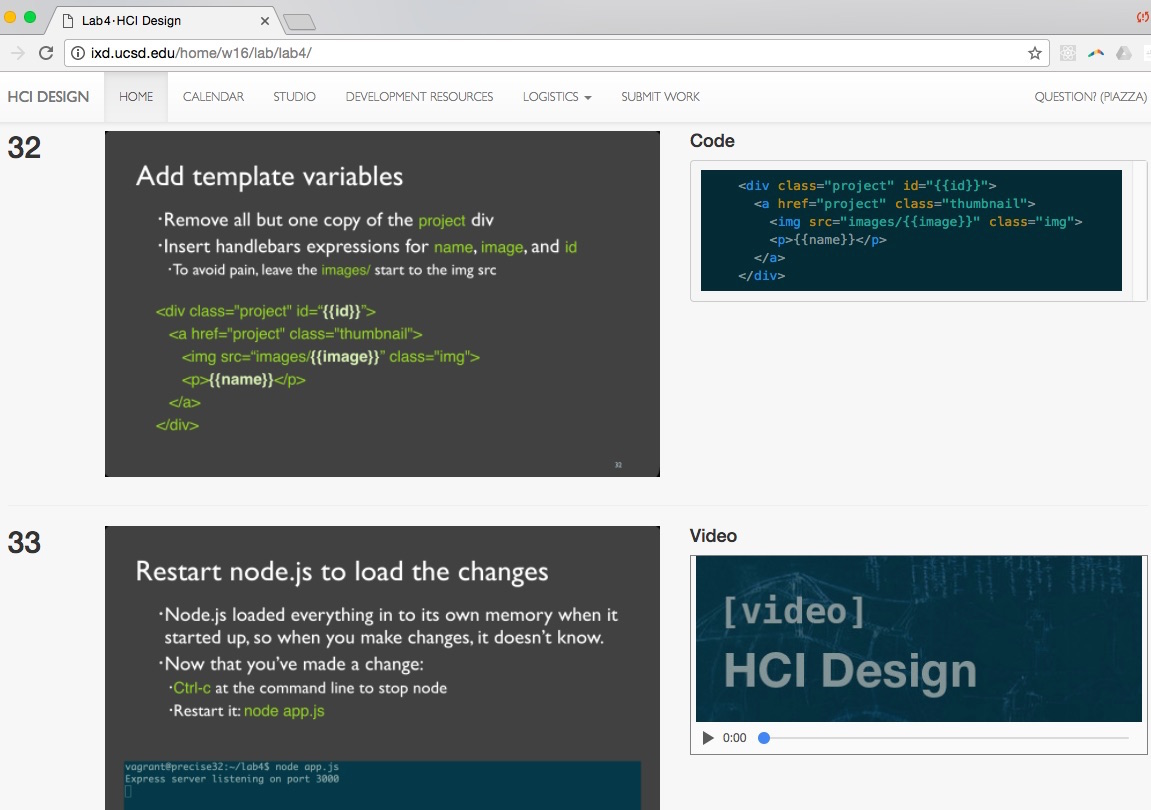
\includegraphics[width=\columnwidth]{figures/torta/ixd-lab-slides.jpg}

\caption{A mixed-media tutorial for web programming that was manually
created for an HCI course~{\protect \cite{ixd}}. Each tutorial is up to
100 steps consisting of PowerPoint slides mixed with code snippets and
videos.}

\vspace{-1em} % stent

\label{fig:ixd-lab-slides}
\end{figure}

To discover the challenges faced by people who manually create
mixed-media software tutorials, we interviewed four teaching
assistants responsible for creating web programming tutorials for an
introductory HCI course~\cite{ixd}.

%Our interviews were semi-structured and focused on walking through their
%process of making, updating, and presenting these tutorials.

In this course, students build full-stack web applications with a mix of
tools such as Git for version control, Node.js for server-side
development, Handlebars for templating, Bootstrap for responsive CSS,
and Heroku for live deployment to the web. Students come into the course
from a diverse variety of majors and widely varying levels of prior programming
experience, so the staff teaches weekly programming tutorials to get
everyone acquainted with the mechanics of web development (e.g., setup,
coding, testing, online deployment). Since these tutorials must
coordinate across multiple command-line and GUI applications, they are
representative of the sorts of tutorials that we would like Torta to
automatically generate.

%Several sets of teaching staff across two universities
%(Stanford and UC San Diego) have iterated on the design of these
%programming tutorials over four years of offering this course and having
%the tutorials used by around 2,000 total students~\cite{ixd}.

Each lesson is a webpage containing a mixed-media tutorial interspersing
PowerPoint slides, video clips, and command/code snippets.
%
Everything is created manually: The staff first makes
a PowerPoint deck (usually around 100 slides) containing step-by-step
instructions, commands to run, code to write/modify, and screenshots
showing expected visual outputs. They export the slides as images to
embed within a webpage and then supplement it with screencast videos and
commands/code that students should copy-and-paste into their terminals.
%
%Students work through the tutorials during class, and the staff walks
%around the classroom to help.
%
From our interviews with teaching assistants, we found three main
bottlenecks in creating these tutorials and deploying them during
in-class lab sessions:

\textbf{\emph{PowerPoint slides versus screencast videos}}: Students
greatly preferred reading the PowerPoint slides since those were easily
skimmable, but the staff found them far more tedious to create since
they needed to first demonstrate their actions and then manually
copy-and-paste all commands, code, expected outputs, and screenshots
into the slides. Also, sometimes the slides did not go into enough
detail or skipped steps due to staff oversight or simply lack of prep time. In contrast, screencast videos were much easier for staff to record and
contain all necessary details, but were harder for students to browse.
The staff struck a compromise by placing slides and videos side by side
on the webpage, using videos to showcase
dynamic events such as GUI interactions and web animations.

\textbf{\emph{Slides, videos, and code are disconnected}}: Besides
slides and videos, the staff also embedded snippets of code and commands
into tutorial webpages. They did this because
students found it hard to copy-and-paste directly from PowerPoint slides
due to syntax-breaking formatting issues (e.g., bad line breaks, smart
quotes, special characters, incomplete code due to lack of space on
slides), and it is impossible to copy from videos. Additionally, the
staff maintained a GitHub repository of skeleton starter code and helper
scripts for students to build upon when following these tutorials. This
heterogeneous setup meant that when the staff created or updated each
tutorial, they had to manually keep four disparate data sources all
updated and in sync:
PowerPoint slides, videos, command/code snippets, and the GitHub
repository of skeleton code; these disconnects led to numerous bugs in
tutorials.

\textbf{\emph{Hard for students to validate progress}}: When working
through tutorials in class, students were anxious about whether they
were following certain steps properly since the PowerPoint slides did
not always specify the expected effects of each step, and videos were
not available for all steps. Many effects were not immediately
visible on-screen, such as the results of running a Heroku configuration
command. Even worse, when a student does not follow a step properly,
everything may still appear to work, but subtle errors silently
propagate and manifest in later steps with unrelated error messages.
These problems arise because students cannot easily check their
progress. The staff ended up dealing with this by writing
\emph{validation scripts} for each tutorial. When a student runs a
validation script, it checks that their filesystem state, environment
variables, and current directory are what the tutorial expects;
otherwise it prints a targeted error message.

%We reflected on the challenges uncovered by our interviews to formulate
These bottlenecks inspired a set of design goals for Torta:

\begin{itemize}\itemsep0pt

\item \textbf{D1}: Creating a tutorial should be as easy as recording a
screencast video, but tutorials should offer advantages of text-based
formats like easy skimming and copy-paste.

\item \textbf{D2}: A tutorial should automatically encapsulate videos,
textual exposition, code examples, and terminal commands together into
one package instead of in disconnected silos.

\item \textbf{D3}: Users should be able to view the tutorial at
varying levels of detail to accommodate their own expertise level.

\item \textbf{D4}: Users should be able to incrementally validate their progress
as they follow each step of the tutorial.

\end{itemize}



\section{The Design and Implementation of Torta}

\begin{figure*}
%\vspace{20em}
\centering
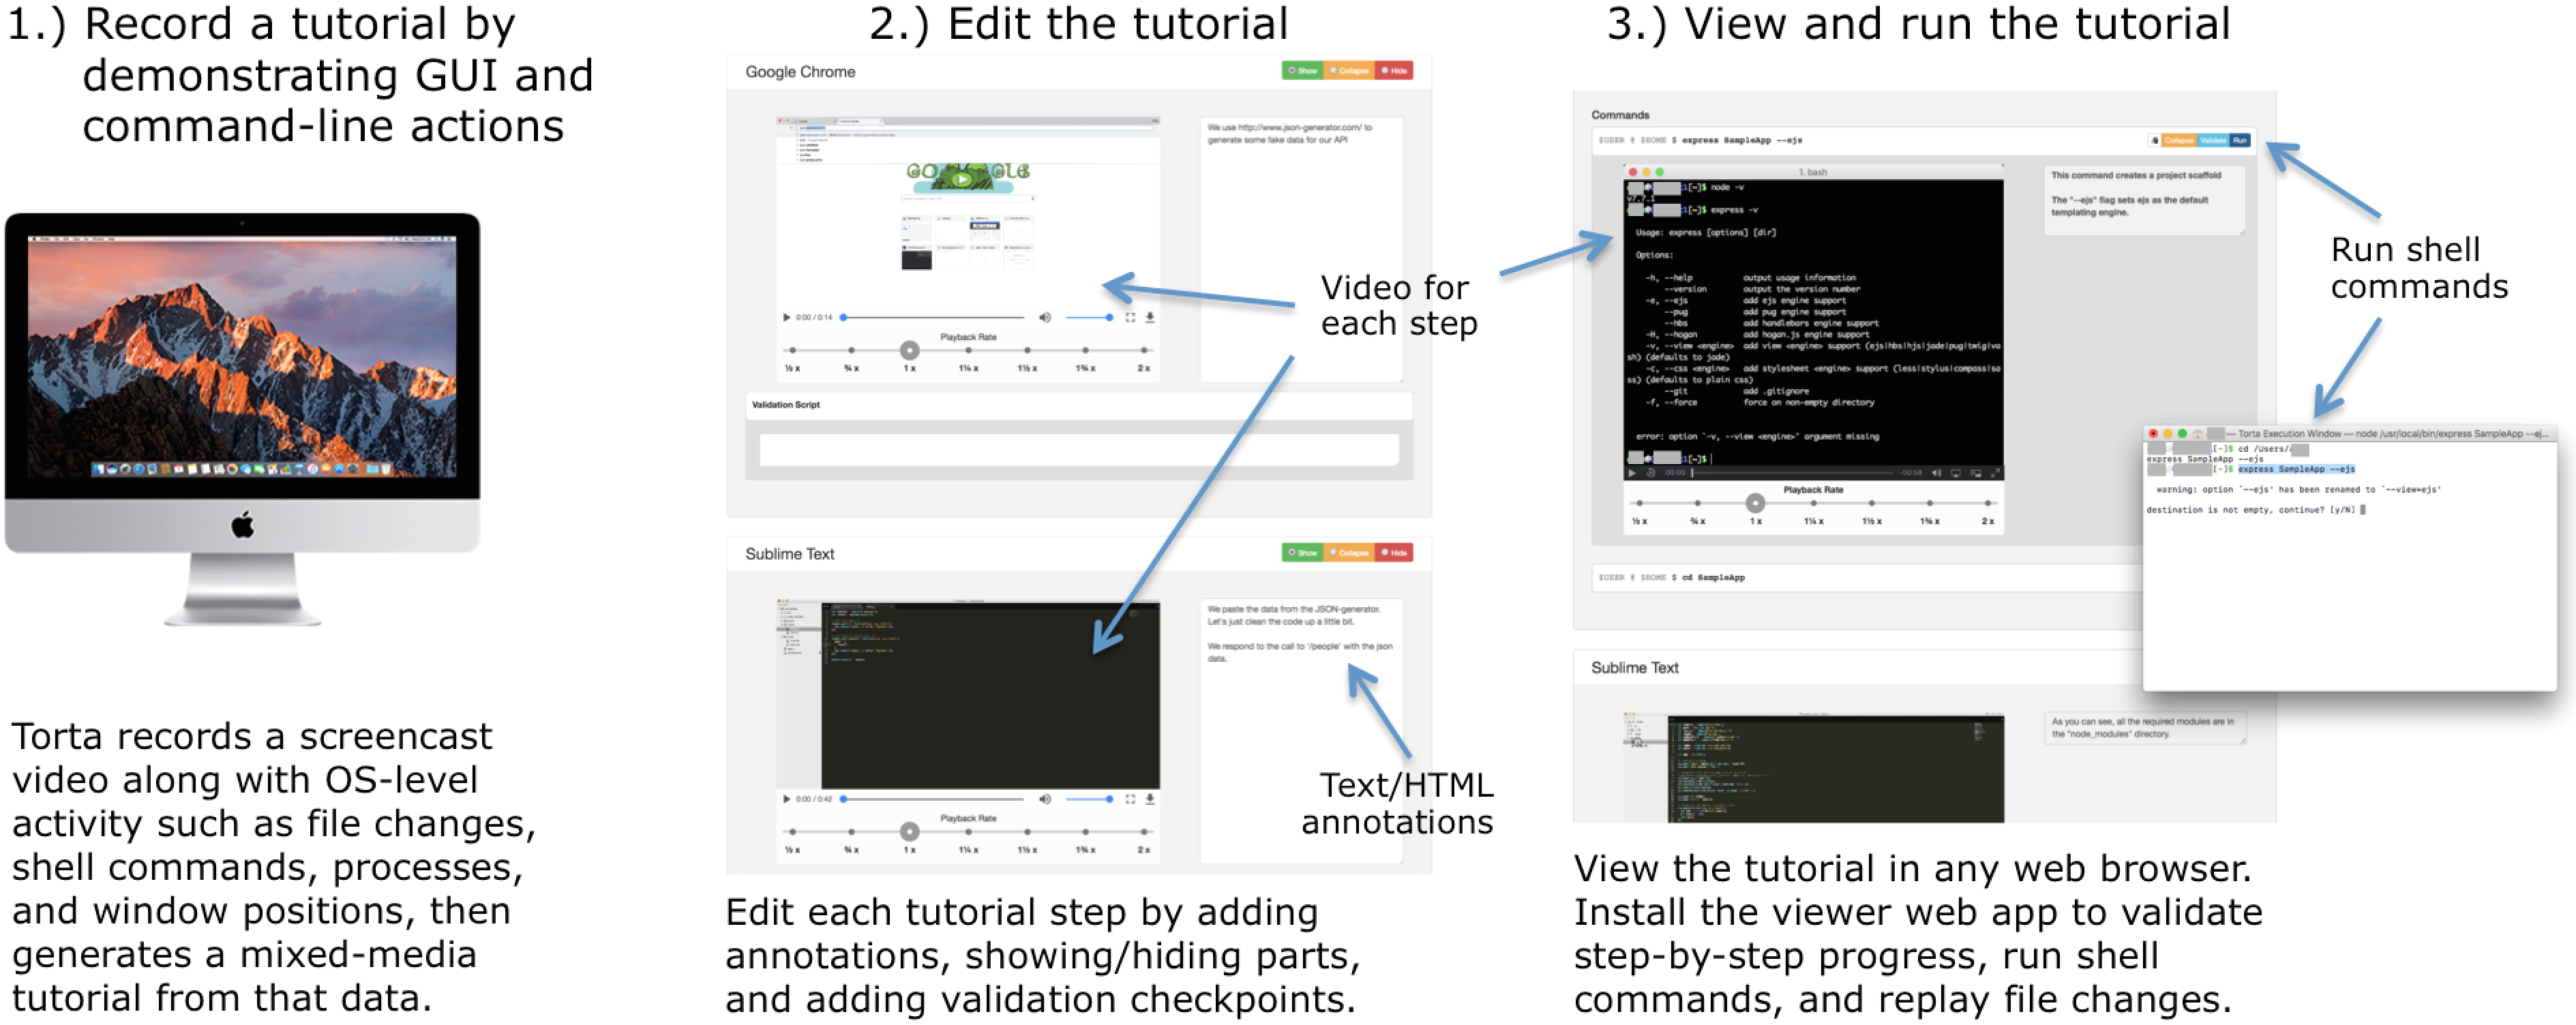
\includegraphics[width=0.98\textwidth]{figures/torta/torta-overview.png}

%\vspace{0.5em}
\caption{Torta allows macOS users to create mixed-media tutorials
by demonstration, and then edit, view, and run those tutorials in a web
browser.}

\label{fig:torta-overview}
\end{figure*}

Torta consists of three components: a tutorial recorder, editor, and
viewer (\fig{fig:torta-overview}). We now describe each in turn.


\subsection{Tutorial Recorder}

Torta's recorder allows the user to record a tutorial just as easily as
recording a screencast video (Design Goal D1).
%
Our prototype is implemented for macOS using AppleScript, Python, Bash,
and DTrace~\cite{Cantrill2004} scripts to perform OS-level activity tracing. It
should be straightforward to port this OS-wide tracing-based approach to other
operating systems.

%such as
%Windows and Linux-based systems since they offer similar kinds of
%scripting and tracing features.

When the user wants to start recording a tutorial, they activate Torta
by running a terminal command, which immediately launches a set of
activity tracers. The user then records their tutorial by simply
demonstrating actions on their computer, and the tracers log the
following data in the background:

\begin{itemize}\itemsep0pt

\item \textbf{Screencast video recorder}: Torta uses Apple's built-in
Quicktime app to record a standard full-screen screencast video with
audio narration and mouse clicks visualized.

\item \textbf{Foreground GUI window monitor}: The position and
dimensions of the user's current foreground GUI window are logged once
per second, along with the process ID of the program that owns the
current foreground window.

\item \textbf{Keystroke logger}: All user keystrokes are logged.

%using Apple's {\small \texttt{CGEventCallback}} events.

\item \textbf{Shell command logger}: The contents of all terminal
commands run in any shell are logged and timestamped. The current
working directory, username, and environment variables used for running
each command are also logged. Our current logger works for Bash (the
default on macOS) and Zsh, but can be easily extended to other custom
shells.

\item \textbf{Filesystem activity tracer}: Torta uses DTrace~\cite{Cantrill2004} to record
a subset of system calls that access the filesystem. Specifically, it
logs the timestamps, owner process IDs, and parameters of the following
filesystem-related system calls: {\small \texttt{open()}}, {\small
\texttt{write()}}, {\small \texttt{close()}}, {\small
\texttt{rename()}}, and {\small \texttt{unlink()}} (for opening, writing
to, closing, renaming, and deleting files, respectively).
Torta makes a timestamped backup copy of each affected file after the
respective system call is run. This feature is useful for saving all versions of
files that users edit within interactive applications such as text
editors, IDEs, or Photoshop: Each time the user presses ``Save" within the app, a
{\small \texttt{write()}} system call occurs, and Torta saves a backup
copy\rev{, which lets it later display diffs}.

\item \textbf{OS process tree logger}: Torta logs the command names,
start/end timestamps, process IDs (PIDs), and parent process IDs (PPIDs)
of all OS processes launched after the user activates Torta. This log
serves two purposes: First, it filters the system call trace (see above)
to consider only processes that launched \emph{after} the user activated Torta,
which eliminates the noise from dozens of irrelevant system-wide
processes previously running on the user's machine. Second, it is
necessary for linking the system call trace to foreground GUI windows.
Here is why: Many interactive apps adopt a multi-process model for
robustness. For instance, Google Chrome launches one OS process per
browser tab, and text editors such as Sublime Text launch one OS process
per text editor tab along with a separate process for the GUI. Thus, the
process that owns the Sublime Text foreground GUI window is \emph{not}
the process that makes the {\small \texttt{write()}} system calls to
save the user's files. Torta can use the OS process tree of
PIDs and PPIDs to link Sublime Text's user-initiated file save events with its GUI
window, since they are owned by sibling processes.

\end{itemize}


\begin{figure}

\centering
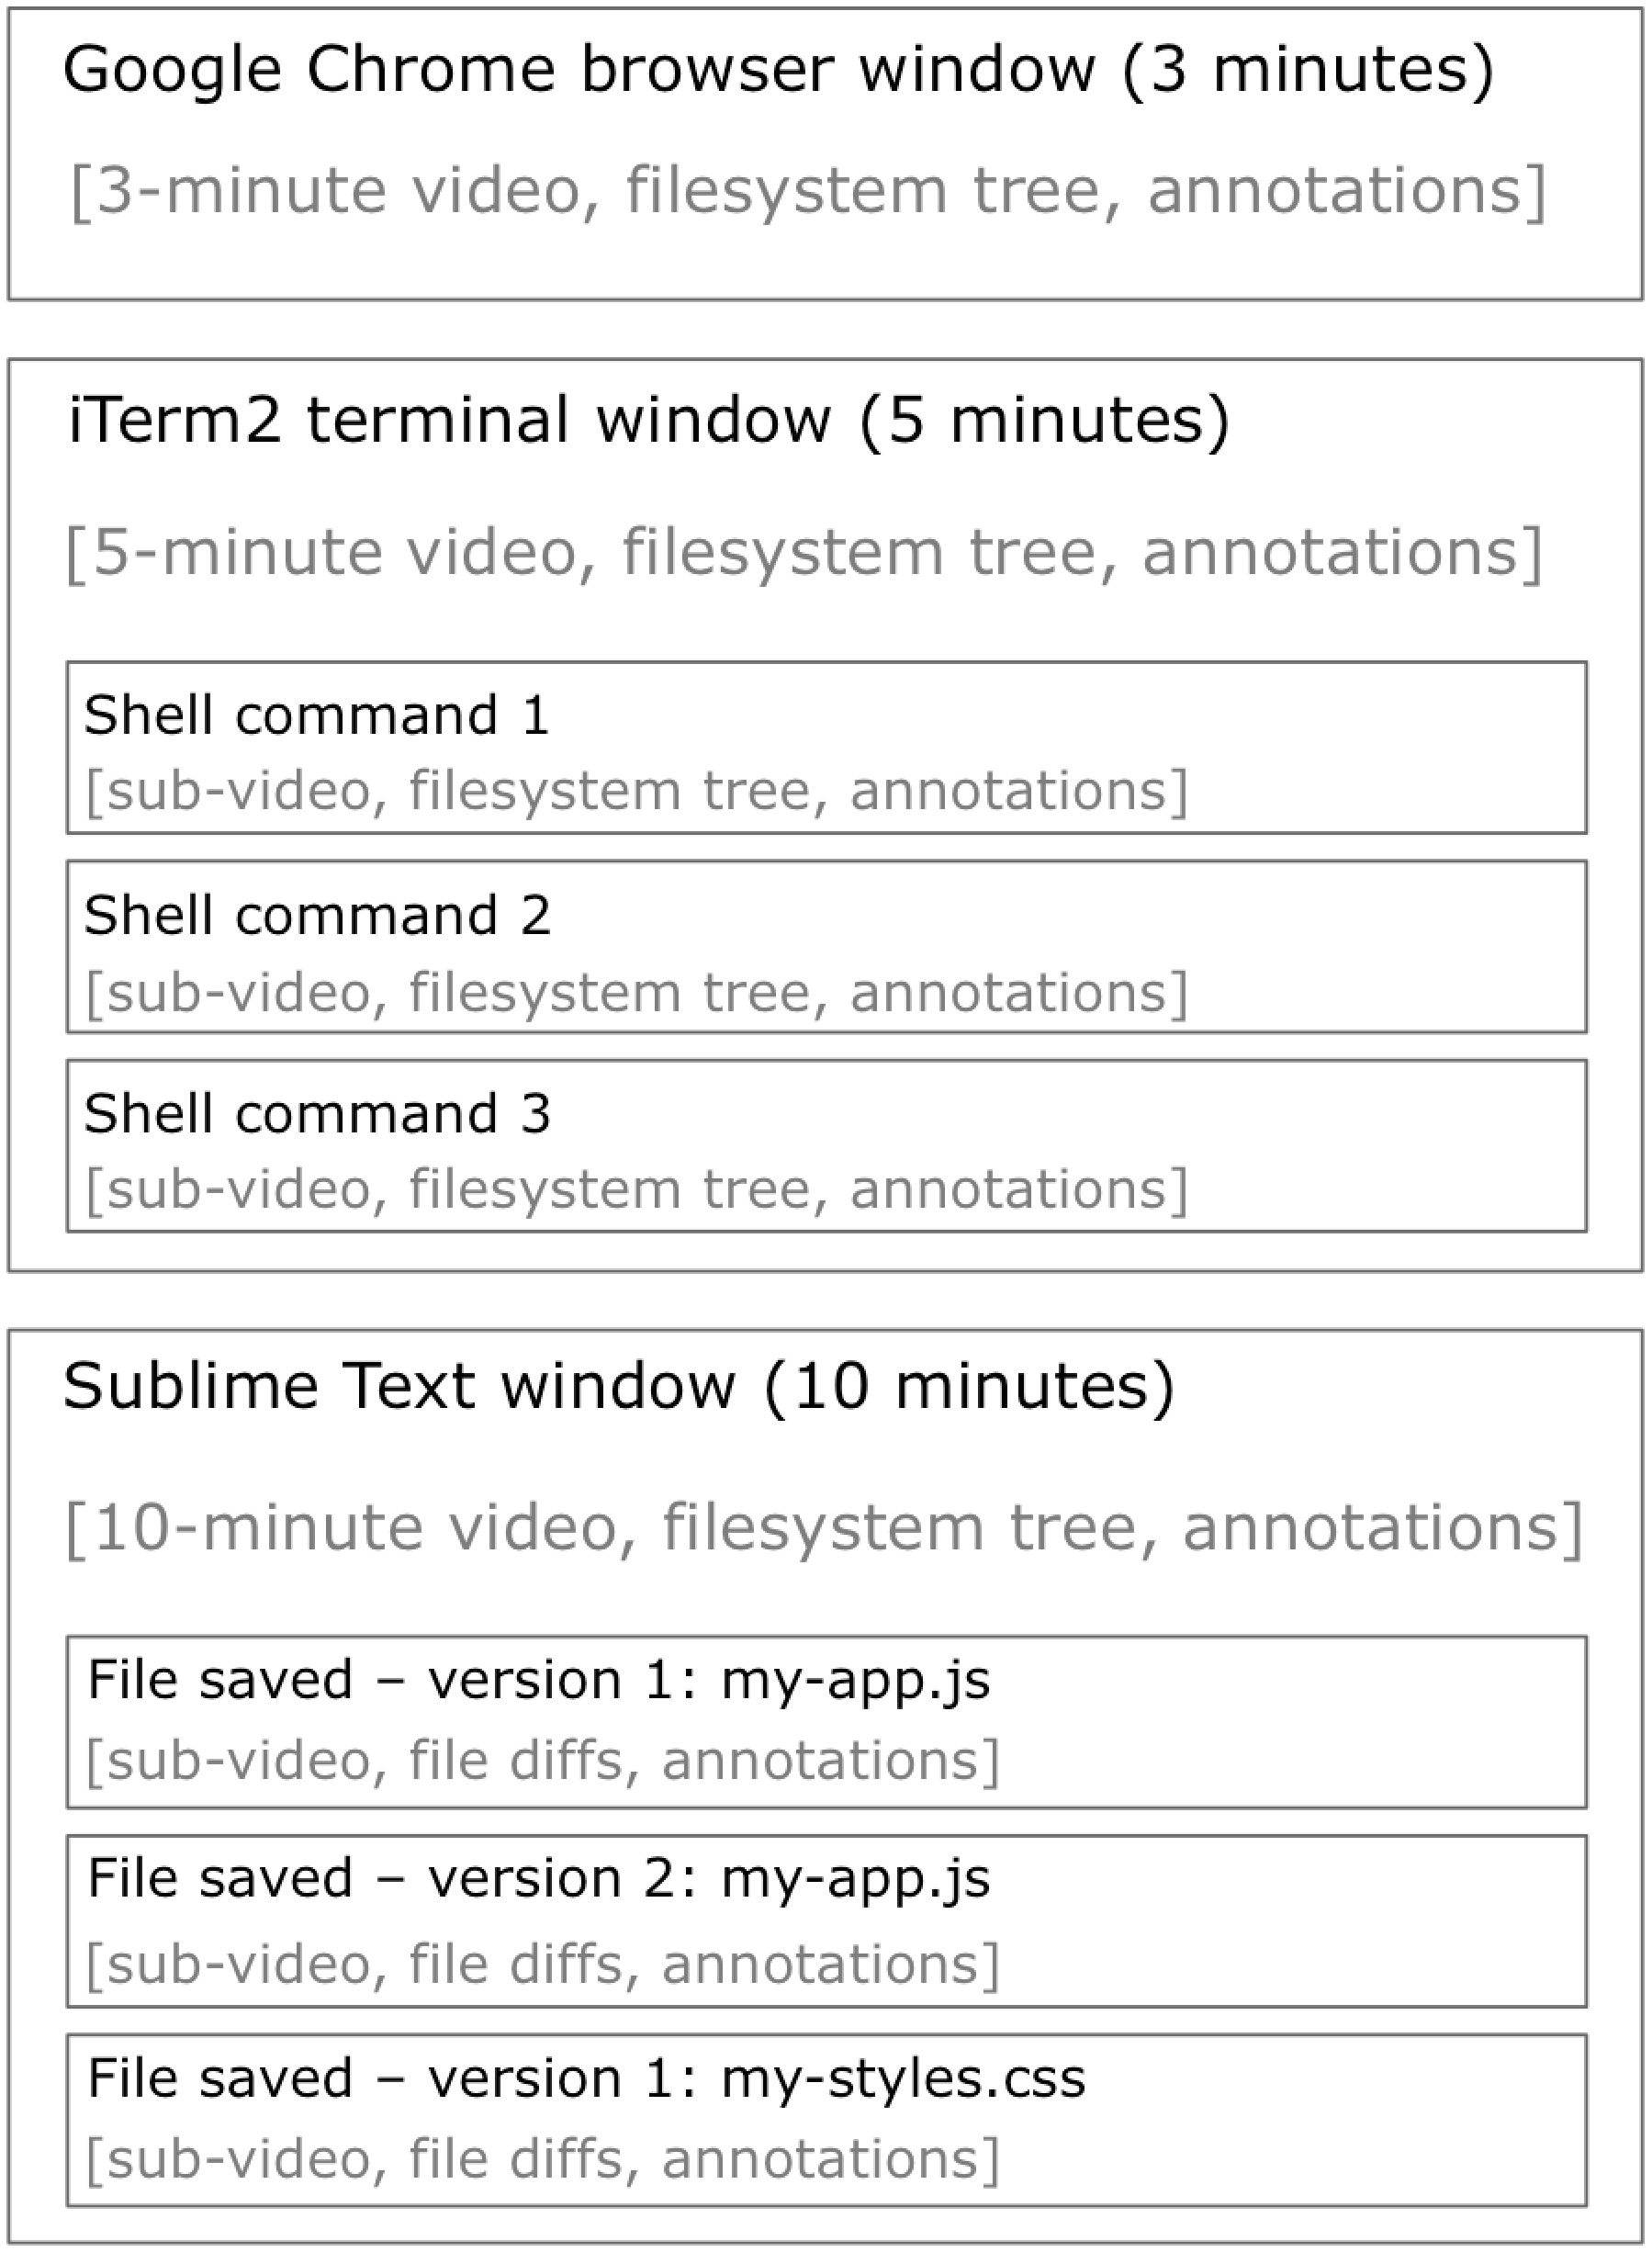
\includegraphics[width=0.85\columnwidth]{figures/torta/torta-schematic.png}

\caption{Example structure of a mixed-media tutorial generated by
Torta. Each of the three steps represents a foreground GUI window duration. There are
three sub-steps within the terminal and IDE windows.}

\label{fig:torta-schematic}
\vspace{-1em} % stent
\end{figure}


\begin{figure*}

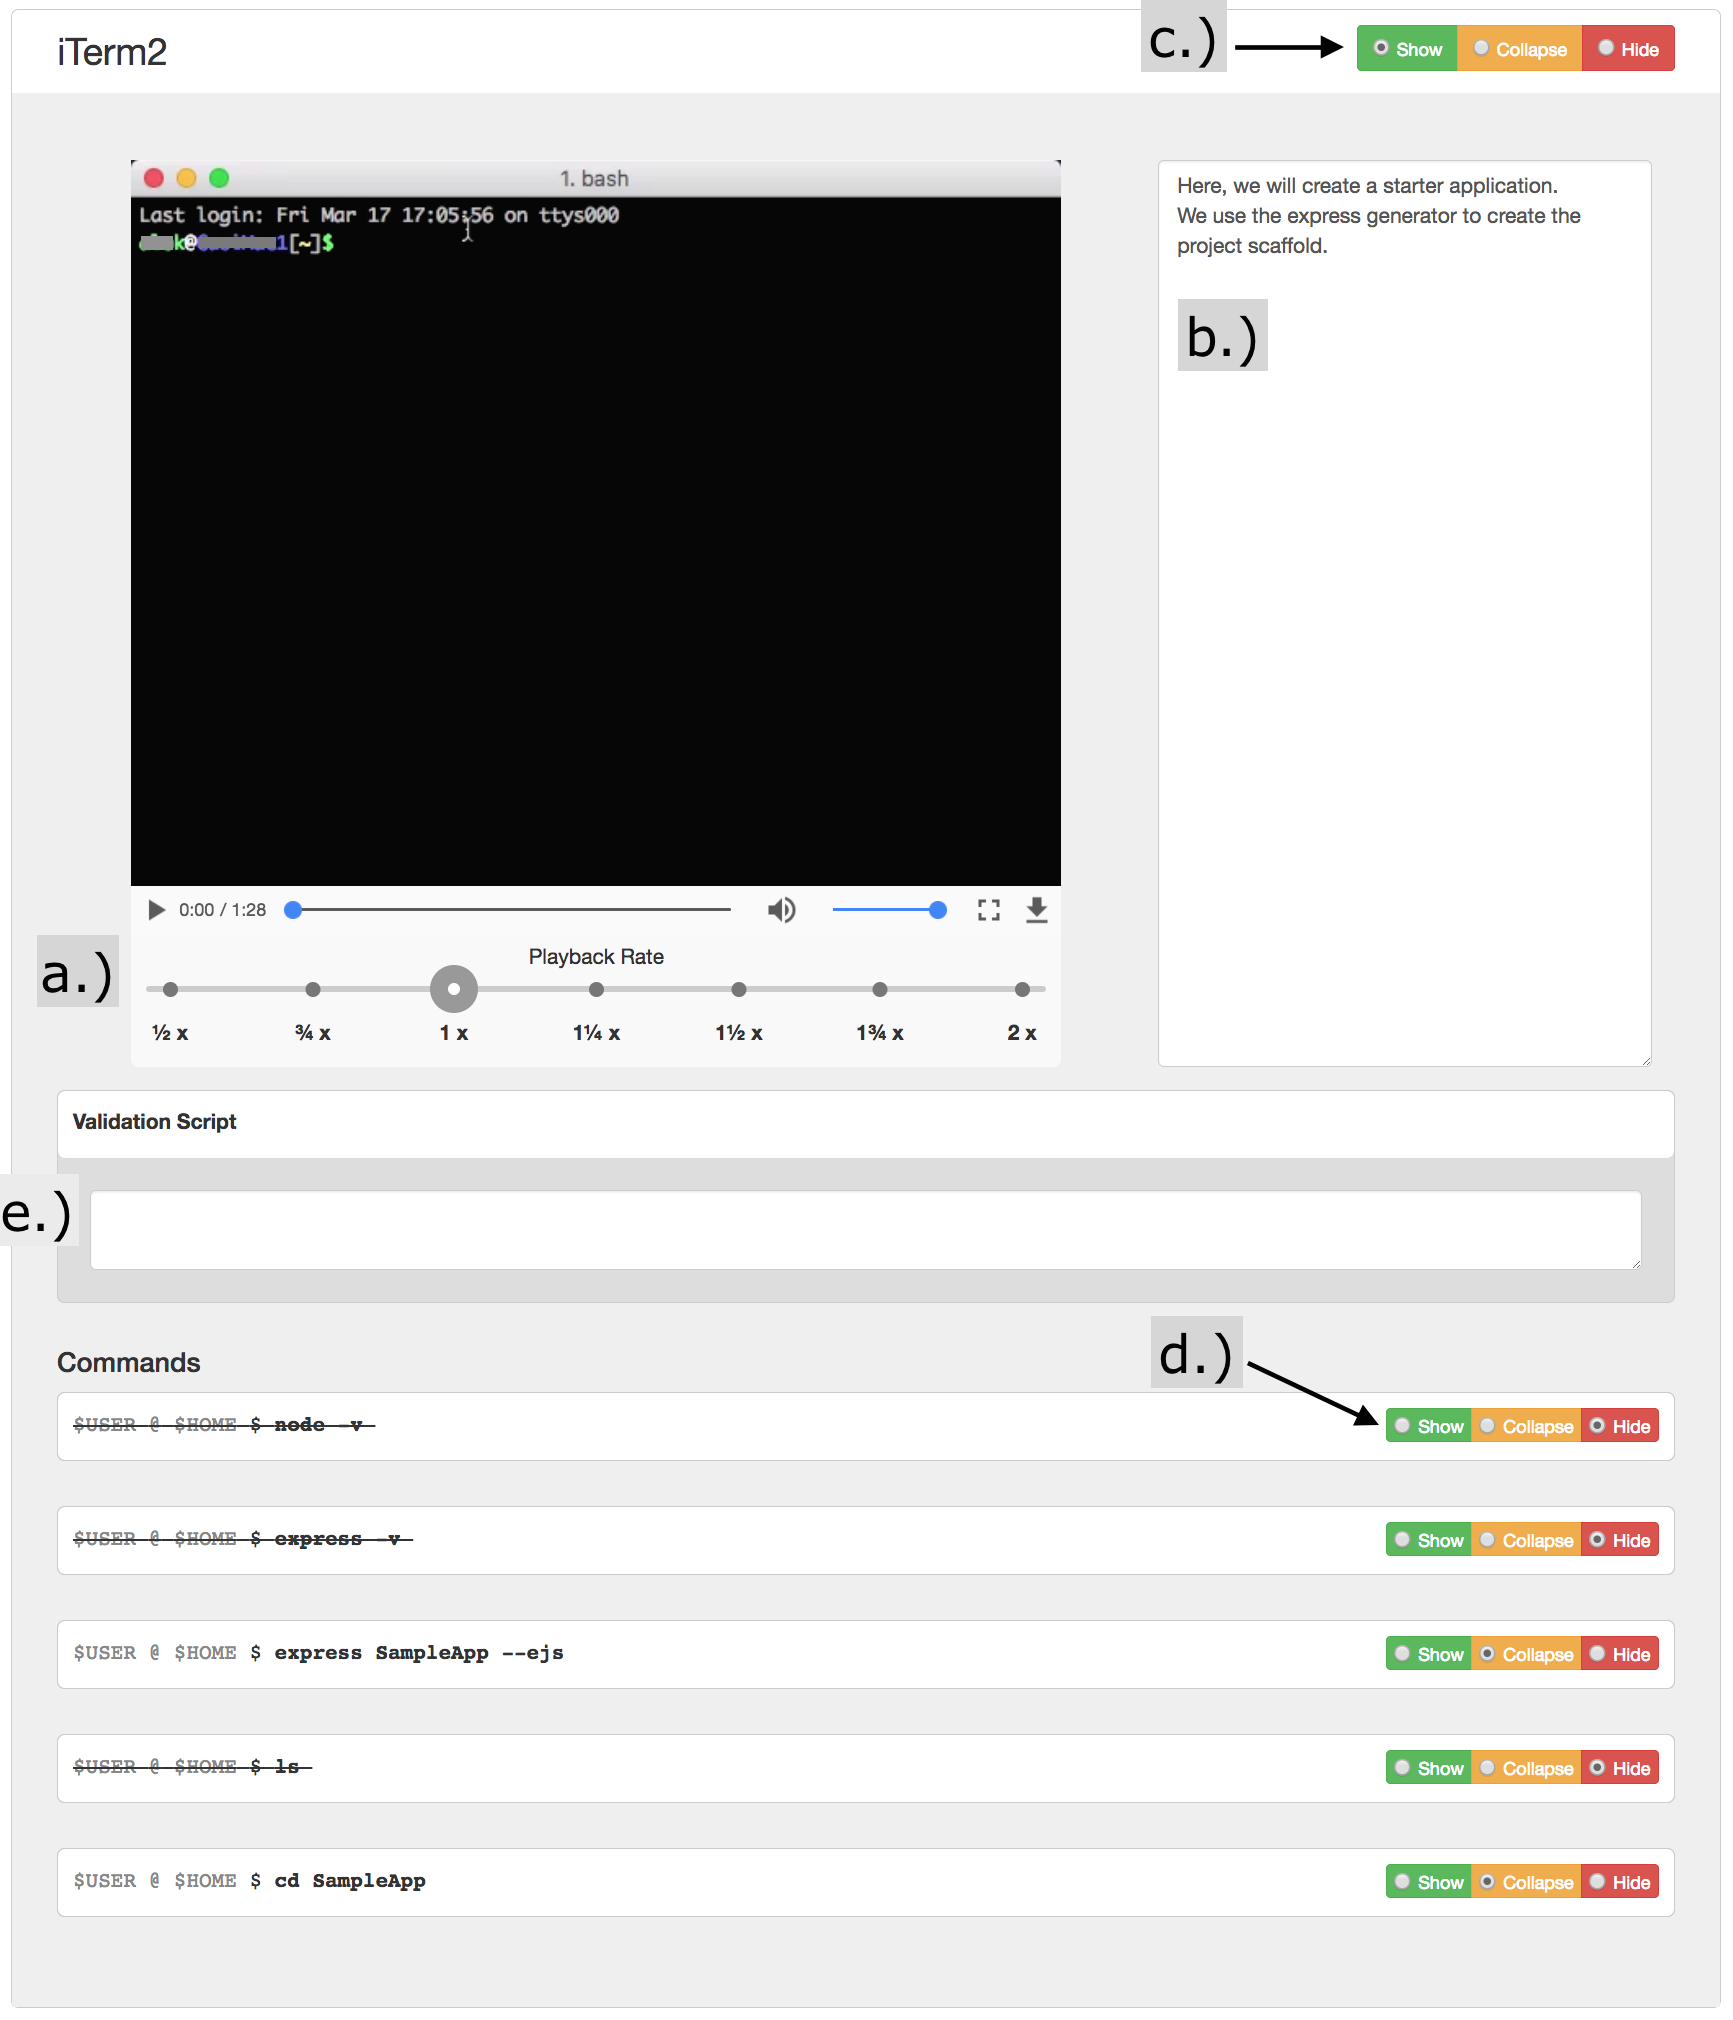
\includegraphics[width=0.488\textwidth]{figures/torta/editor-iterm2.png}
\hspace{6em}
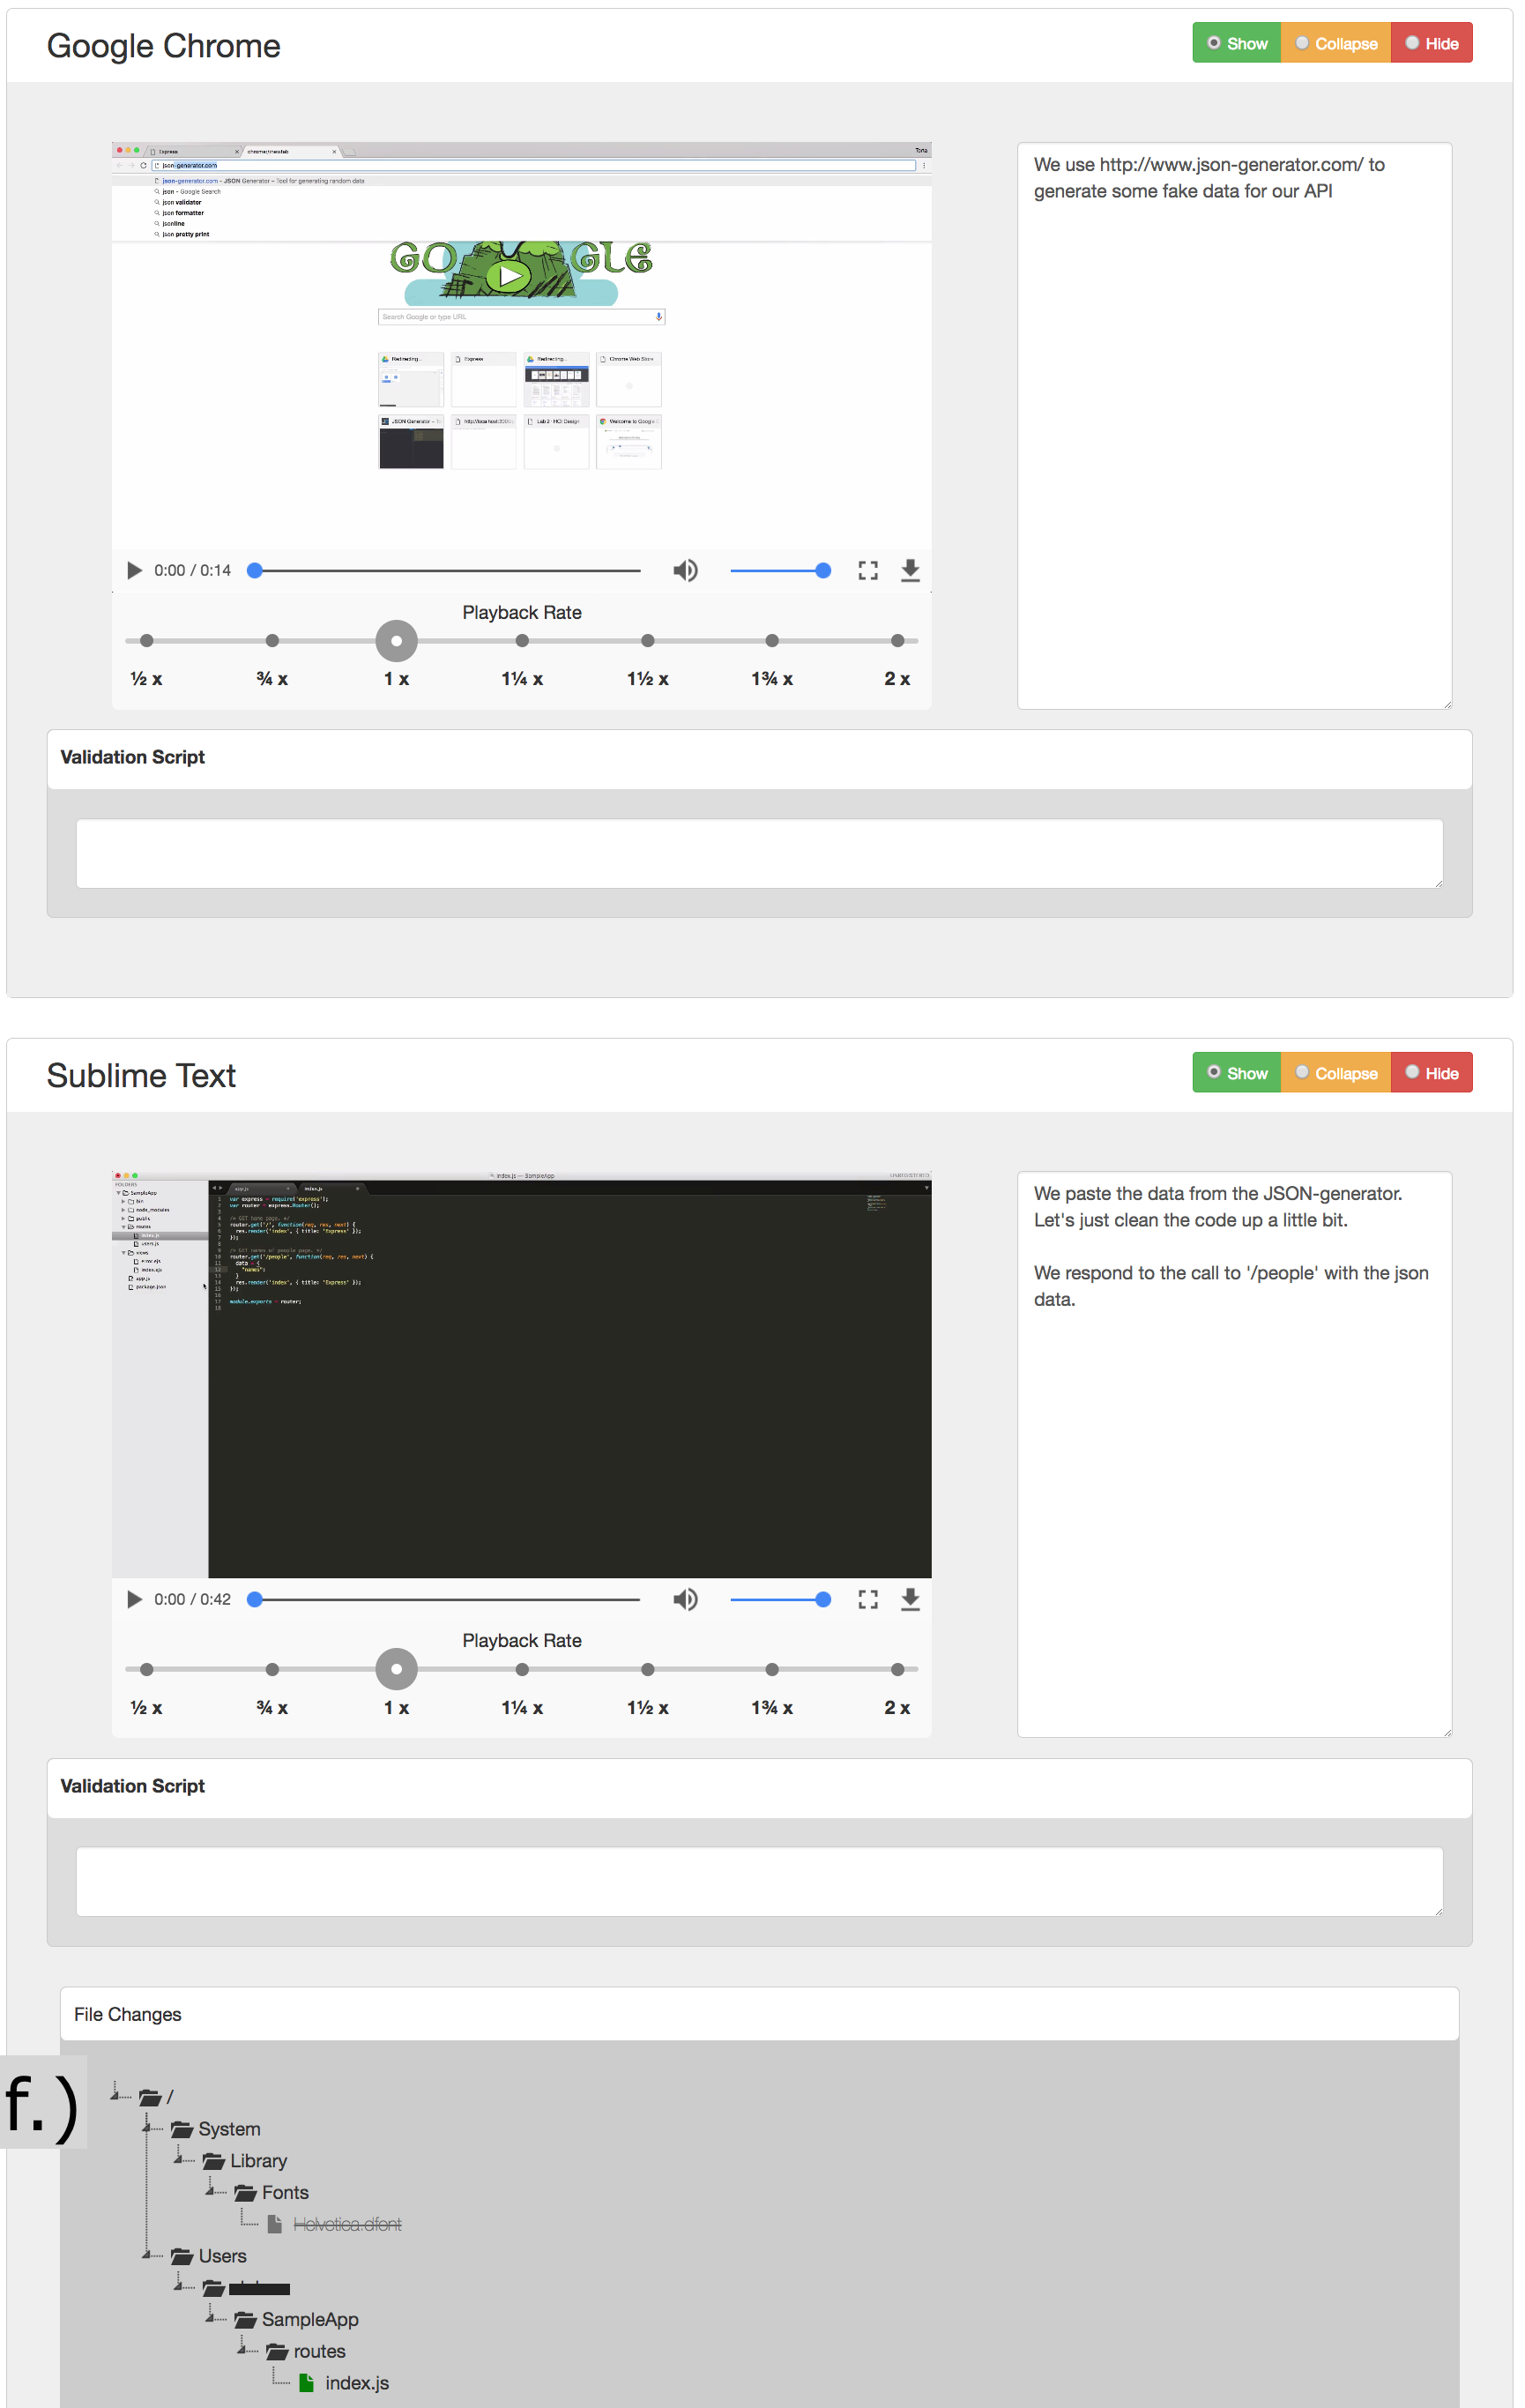
\includegraphics[width=0.359\textwidth]{figures/torta/editor-sublime-chrome.png}

\caption{Zoomed-in screenshots of Torta's tutorial editor showing three
steps (i.e., foreground windows): iTerm2, Google Chrome, and Sublime
Text. Each step contains:
a.)~Video player with playback speed adjuster,
b.)~Text annotation box,
c.)~Toggle to show/collapse/hide this entire step,
d.)~Toggle to show/collapse/hide each sub-step (here the hidden shell command
sub-steps are crossed-out),
e.)~Validation script,
f.)~Filesystem tree (see \fig{fig:torta-fstree}).}

\label{fig:torta-editor}
\end{figure*}


%Throughout testing, we did not observe any noticeable
%run-time slowdowns from these tracers. The one exception was that we
%originally used FSEvents and OpenSnoop to trace filesystem activity, but
%those ended up being too slow and memory-intensive. We quickly switched
%to DTrace, which was much faster since it was designed for
%efficiency~\cite{Cantrill2004}.

After the user finishes recording their demonstration and shuts down
Torta, it automatically creates a \emph{mixed-media tutorial} by
post-processing and combining the recorded data  into self-contained
package that contains all traces, segmented videos, and saved file
versions (Design Goal D2). As shown in \fig{fig:torta-schematic}, a
Torta-generated tutorial has a hierarchical structure that aims to
follow the design guidelines of Chi et al.~\cite{Chi2012}:


\textbf{Top-level steps -- foreground GUI windows}: A Torta tutorial is
an ordered list of top-level steps. Each step spans the duration of one
foreground GUI window. Torta uses FFmpeg~\cite{ffmpeg} to split the screencast video into
one mini-video per foreground window duration and crops those videos to
show only the foreground window. We felt that foreground windows were
the most natural step boundaries for these kinds of software
tutorials, since users often perform a set of actions within one window
(e.g., an IDE) and then switch to another window (e.g., Photoshop) to
perform the next set.

Each step is rendered as a mini-video along with a \emph{filesystem
tree} showing which files were added, deleted, renamed, and modified by
processes associated with the foreground GUI window during that step
(\fig{fig:torta-fstree}). We chose to visualize filesystem changes since
those represent the persistent effects of user actions within an
application. Regardless of what kind of app the user is running, if some
action has a lasting effect on their computer, it will likely manifest
in the filesystem.


\textbf{Sub-steps}: Torta further splits each top-level step into
sub-steps based on two common kinds of user actions
(\fig{fig:torta-schematic}):

\begin{itemize}\itemsep0pt

\item \emph{\textbf{Shell commands}}: If the user runs multiple shell commands
within the duration of one foreground window (usually some kind of
terminal app), Torta splits that step into one sub-step for each command.
Each sub-step is shown as a mini-video spanning the duration of only
that command, the text of that command, its current working directory,
environment variables, and a filesystem tree showing what files that
command added, deleted, renamed, and modified.

\item \emph{\textbf{File saves}}: When the foreground window is an
interactive app such as an IDE, web browser, or image editor, the user
may be editing files and periodically saving their progress to disk.
Torta splits each step into sub-steps based on file save events,
treating saves like user-defined checkpoints in the tutorial. Again,
each sub-step gets its own mini-video. If the saved file is plain text,
Torta also shows the diffs between the current and previously-saved
versions, which is useful for showing edits in code and configuration
files. 

%\todo{how does Torta differentiate these file saves from the files
%mutated by a shell command shown above?!?}

\end{itemize}

%Torta bundles the entire tutorial -- all filtered traces, segmented
%videos, and saved file versions -- into a self-contained package that
%can be deployed to the web (Design Goal D2).


\subsection{Tutorial Editor}

The mixed-media tutorial that Torta automatically generates from the
user's demonstration is already complete and ready to view on the web.
One can think of it as a screencast video that is segmented and
enhanced with OS-level trace data. However, it can be hard
for users to record a pristine, error-free video in one take.
Furthermore, users also want to augment tutorials with textual
annotations and other customizations. To fulfill these needs, Torta
provides a tutorial editor,
%
which renders the tutorial just as the viewer would see it but
adds extra controls for the following actions (\fig{fig:torta-editor}):

\textbf{Adding text annotations to steps/sub-steps}: The user
should already provide audio narration when recording their
demonstration, which will show up in the screencast video. The editor
also lets them add Markdown-based rich-text annotations next to the segmented video for
each step/sub-step.
%These annotations support Markdown, which is useful
%for adding web links.
%
%In the future, we could hook Torta to an automated or crowd-based
%transcription service to automatically convert audio narration into
%textual annotations.

\textbf{Hiding steps/sub-steps}: The user can hide any step/sub-step
from the viewer to eliminate mistakes or redundancies (effectively
deleting them from the edited tutorial). If the user hides a step that
is in between two steps that belong to the same application, then those
two surrounding steps get merged into one. This happens when, say, the
user is in an IDE, then switches to a web browser to look up something
quickly, then switches back to the IDE. If the user hides the web
browser step because they deem it irrelevant for the tutorial, then the
two IDE steps get merged together as one step in the viewer.
%
\rev{Torta does not support post-hoc re-recording of steps in the
editor. A workaround is to record an entire session even with errors
included and then hide erroneous steps using the editor.}

%(Note that we did not implement reordering of steps since it rarely
%makes sense to change the order of actions within a software tutorial.)

\textbf{Collapsing steps/sub-steps}: If the user deems certain steps or
sub-steps to be less important for the tutorial, they can show them in a
collapsed form. The viewer will see those steps as a collapsed summary
but can manually un-collapse them to dive into details. Torta displays
compact summaries so that viewers can more easily skim step contents
(e.g., ``Photoshop window active for 2 minutes, modified 3 files").

Torta implements heuristics to automatically collapse certain
steps/sub-steps that are likely to be less important to the tutorial.
For instance, if a shell command does not make any changes to the
filesystem (e.g., {\small \texttt{ls}} or {\small \texttt{git status}}),
it is collapsed by default since the user was probably checking their
setup before proceeding to the next step. Also, if any GUI window was in
the foreground for less than 5 seconds, had less than 10 user
keystrokes, and did not modify the filesystem, then its step is also
collapsed by default. This filters out ``flickers" where the user
switches between windows momentarily to quickly check something before
the next step.
%
%Note that these also make good candidates for deletion, but it is up to
%the user to make the final decision to delete.

\begin{figure}

\centering
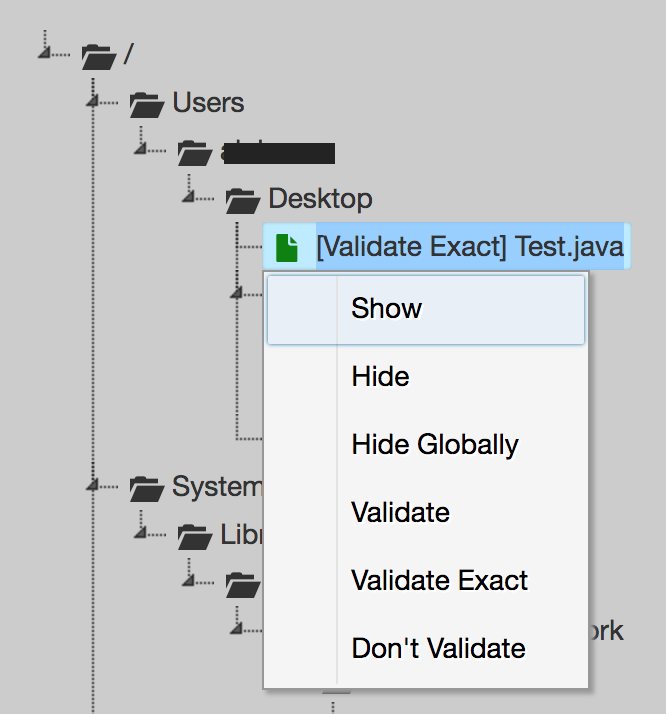
\includegraphics[width=0.56\columnwidth]{figures/torta/filesystem-tree.png}

\caption{Each file-modifying tutorial step displays a filesystem tree of
all files affected by running that step. In the editor UI, the user can
right-click to show/hide files and to mark for validation.}

\label{fig:torta-fstree}
\vspace{-0.5em} % stent
\end{figure}


\textbf{Collapsing filesystem tree components}: Recall that Torta
displays a filesystem tree within each step and
sub-step that modifies the filesystem (\fig{fig:torta-fstree}). However,
during pilot testing we
noticed that some commands (e.g., {\small \texttt{git clone}}) can
affect hundreds of files, so their trees are extremely large. To reduce
visual overload, the user can collapse tree nodes to hide and summarize
their sub-trees. For instance, the user can
collapse a {\small \texttt{.git/}} sub-directory to see a summary like
``100 files added and 15 files modified in \texttt{.git/}." Just as with
collapsed steps, the viewer can un-collapse tree nodes to see more details
on demand. The user can also choose ``Hide Globally" to hide a
particular file/directory across all tutorial steps.

%\textbf{Changing video playback speed}: Users can adjust the default
%playback speed for each video from 0.5X to 2X.

%Viewers can override the defaults if desired.

\textbf{Adding validation}: The editor provides two ways to specify how
people (i.e., tutorial \emph{consumers}) can validate progress at each
step as they are following the tutorial (Design Goal D4):

\emph{\textbf{1.~Marking files to validate}}: The user can mark each
file in the filesystem tree of a step/sub-step as ``Validate",
``Validate Exact," or ``Don't Validate" (\fig{fig:torta-fstree}). If the user marks a directory,
everything within it also gets marked with that label. ``Validate" means
that Torta should check that the consumer's file gets altered in the way
that this step specifies (e.g., modified or renamed), and ``Validate
Exact" means that the new contents of the file should also exactly match
the saved version bundled in the tutorial package. For example, in a step where the consumer is supposed
to add their username to a section within a configuration file, that
file should be marked as ``Validate" to check that it has been modified,
but not ``Validate Exact" since everyone's username will be different.

\emph{\textbf{2.~Writing validation scripts}}: File-based validation
handles the most common uses, but if tutorial creators want more
flexibility, they can write a validation script for each
step/sub-step (\fig{fig:torta-editor}e). This is a Bash script that will run on the consumer's
machine to check that their OS state is as expected.

\rev{This feature is similar in spirit to the step-level validation
features offered by tutorial systems for other
domains~\cite{Fernquist2011,Pongnumkul2011}}.

After the user finishes editing the tutorial, they can publish it as a
webpage or send the self-contained package to viewers.


\subsection{Tutorial Viewer}

Since Torta tutorials are ordinary webpages, they can be viewed in any
browser. Each tutorial initially loads with certain steps/sub-steps
collapsed, certain file tree nodes collapsed, and each video playing at the
speed pre-set by the creator. However, the user can adjust any of those
settings. In addition, they can click on any file in the tutorial and
view/download the version of that file present during that respective
step (all versions are stored in the package). This ability to
selectively hide and show details was inspired by a challenge discovered
during formative interviews: Students preferred seeing varying levels of
detail depending on their expertise level (Design Goal D3). It is hard
to achieve this flexibility with raw screencast videos or PowerPoint
slides.

To make tutorials more readable, Torta canonicalizes all file paths
within command invocations and filesystem trees. For instance, when
Alice creates a tutorial, many of her file paths will contain {\small
\texttt{/home/alice}} if they are within her home directory. But when
Bob is viewing the tutorial, he would prefer to see paths starting with
{\small \texttt{/home/bob}} instead of {\small \texttt{/home/alice}}.
Torta canonicalizes paths by replacing the creator's home directory with
the \texttt{\$HOME} variable. Additionally, the creator can use the
tutorial editor to specify other path variables to replace. One use case
is specifying a \texttt{\$PROJECT\_ROOT} directory where all files
within a project should live. The tutorial viewer prompts the user to
enter their own preferred values for all of these variables and rewrites
all paths within the webpage accordingly. Note that \texttt{\$HOME} and
other environment variables are automatically set if the tutorial is
loaded from the user's machine rather than viewed on the web.


\begin{figure}

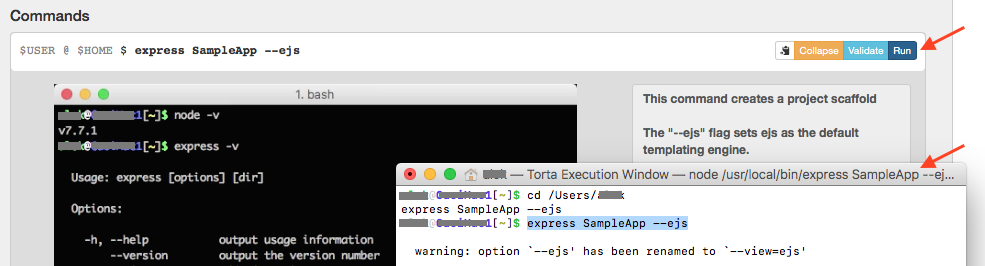
\includegraphics[width=\columnwidth]{figures/torta/view-and-run.png}

\caption{Each step and sub-step contains ``Validate" and ``Run" buttons
on the upper right. Here when the user clicks on ``Run" for a shell
command sub-step, Torta runs that commands in a new terminal window.}

\label{fig:torta-player}
\vspace{-1em} % stent
\end{figure}


If the user downloads the tutorial to their macOS machine and loads it
via the Torta viewer web app on localhost, then they can access two additional features as shown
in \fig{fig:torta-player}:

\emph{\textbf{1. Validating step-by-step progress}}: After manually
performing the actions specified by a particular step/sub-step, the user
can click the ``validate" button alongside its video. Torta will check
that the affected files on the user's local filesystem have been
modified in the ways that the creator originally expected (i.e.,
specified via ``validate" and ``validate exact" labels in the filesystem
tree) and also run the validation script if it exists. Then it prompts the user if
there are errors and offers to overwrite any mismatched files with
the versions from the tutorial package if the user wishes. This
capability lets the user check that they are properly following along
with each step of the tutorial and to catch bugs earlier (Design Goal
D4).

\emph{\textbf{2. Automatically running steps}}: The user can click the
``run" button next to each step/sub-step to have Torta automatically run
that step for them.  For a shell command, Torta launches a terminal
app on the user's machine and runs the command from that terminal after
setting the proper working directory and environment variables. For a
step involving a GUI application, Torta does not try to replay GUI
actions but rather simply mutates the user's filesystem in the way that
has been prescribed by that step. Although this approach is not
always guaranteed to be fully faithful to that step's actions, in practice it
works well in some cases since the persistent effects of a GUI
application usually manifest in the filesystem. For instance, if someone
demonstrates how to use a GUI to customize the configuration of a
complex interactive application, the effects of that customization
may show up as changes to some config file. When the user hits
``run" on that step, Torta simply copies over the updated version of that
config file.

\begin{table*}[h]
\small
\centering
\begin{tabulary}{\textwidth}{@{}LLLCCCCCCC@{}}
& First & Tutorial Topic & GUI Apps & Command-line Apps & Torta Time (recorder+editor) & \# Torta Steps (before edits) & GDocs Time & \# GDocs Steps \\
\hline
S1  & GDoc & HTML and CSS web design & Finder, Sublime Text, iTerm2, Google Chrome & node, touch & 14m (8+6) & 8 (11) & 30m & 7 \\
\hline
S2  & GDoc & Node.js server setup and API endpoint creation & Finder, Sublime, iTerm2, Chrome, Postman & npm, express, node, touch & 15m (7+8) & 12 (14) & 24m & $\dagger$ \\
\hline
S3  & GDoc & JavaScript frontend web dev & Finder, Sublime, iTerm2,Chrome & python & 17m (12+5) & 12 (16) & 32m & 8 \\
\hline
S4  & GDoc & Data science: neural nets w/ Keras and TensorFlow & Finder, Sublime, iTerm2 & python, pip & 19m (11+8) & 3 (8) & 38m & 3 \\
\hline
S5  & GDoc & Data science: linear regression w/ scikit-learn & Finder, Sublime, iTerm2, Chrome & python, pip, brew & 15m (12+3) & 5 (8) & 43m & 5 \\
\hline
S6  & Torta & Go language toolchain install and setup & Finder, Sublime, iTerm2 & gcc, make, cat, golang, brew & 31m (21+10) & 13 (18) & 32m & 10 \\
\hline
S7  & Torta & Java singly-linked list & Finder, Netbeans, iTerm2 & javac, java & 25m (15+10) & 6 (7) & 28m & 5 \\
\hline
S8  & Torta & C doubly-linked list & Finder, iTerm2, Chrome & gcc, vim & 27m (22+5) & 6 (10) & 24m & 4 \\
\hline
S9  & Torta & Python list comprehensions & Finder, PyCharm, iTerm2 & python & 16m (10+6) & 4 (7) & 23m & 5 \\
\hline
S10 & Torta & C binary search tree & Finder, iTerm2, Chrome & gcc, vim & 29m (21+8) & 10 (15) & 30m & 10 \\

\end{tabulary}

\caption{Tutorial creator study results, showing subject IDs, which tool they used first, summary of their tutorial, time in each tool, and the numbers of steps in Torta and GDoc tutorials ($\dagger$ did not explicitly denote steps in GDocs). All times reported in minutes, with Torta split into recorder+editor times.}

\vspace{-1em} % stent
\label{tab:creator-study}
\end{table*}

\section{\rev{Exploratory User Studies}}

\rev{As a first pass at illustrating Torta's capabilities, we compared
users' experiences} of both creating and consuming Torta tutorials to doing
so with manually-written tutorials. We chose to \rev{initially} compare Torta to manually-written
text+screenshot tutorials since those are now ubiquitous on the web in the
form of technical blog posts, documentation websites, \rev{PowerPoint
presentations}, course lecture
notes, Q\&A and forum posts, and (electronic+paper) books.
%
\rev{Note that although we compared with written tutorials for this
exploratory study, a more rigorous controlled study would have also compared
Torta to recording and editing screencast videos, since that is a closely-related
and also-ubiquitous format for tutorials.}

To cover the two target audiences for Torta, we ran two \rev{exploratory} user studies:
1)~A study on tutorial creators, which tests Torta's recorder and
editor components, and 2)~a study on tutorial consumers, which tests Torta's viewer app.


\subsection{Tutorial Creator User Study}

First we compared the \rev{user experience} of creating a tutorial with Torta
versus manually writing a tutorial in Google Docs. We chose Google Docs
since it is a convenient way for someone to quickly create a written tutorial; it
supports rich text formatting, copy-and-paste of screenshot images, and
does not require specialized knowledge of HTML or other markup
languages. \rev{(Microsoft Word would have worked just as well.)}

\emph{\textbf{Procedure}}: We recruited 10 graduate students who have
served as teaching assistants (TAs) for computer science courses to each
perform a 1.5-hour lab study using both Torta and Google Docs on a 21.5"
iMac. We told each subject to create a multi-application software
tutorial for a relevant topic from a class that they have TA'ed. To
counterbalance tool order, we had five subjects first spend up to 40 minutes
creating their tutorial in Google Docs, then try to
re-create that \emph{same tutorial} in Torta. We had the other five
subjects use Torta first, and then re-create the same tutorial in Google
Docs.

Right before each subject used Google Docs, we encouraged them to design a
well-structured step-by-step tutorial with a mix of text, screenshots,
and formatted code/command snippets in monospaced font to emulate a
technical blog. Right before each subject used Torta, we gave
them a five-minute tutorial (a ``Tortorial") on Torta's recorder and
editor UIs.

We spent the final 10--20 minutes of each session conducting a
semi-structured interview where we had the subject compare their
experiences using Torta and Google Docs then self-assess the quality of
the tutorials they created in both tools.


\emph{\textbf{Results}}: \tab{tab:creator-study} summarizes the
generated tutorials. All involved multiple GUI and command-line apps
such as IDEs, compilers, build tools, package managers, and webservers.
%
All subjects used the Torta editor to eliminate a few steps that arose
from errors in their recording (the ``before edits" entries in
\tab{tab:creator-study}). They also collapsed ``boring-looking" steps
such as restarting the Node.js server repeatedly. However, they did not
write many textual annotations due to lack of time and because they
had already recorded voice narration in videos.

During the post-study interviews, all
10 subjects self-reported that they preferred using Torta over Google
Docs (GDocs). They also all
self-reported that they felt their Torta-generated tutorials were better organized
and higher quality. Multiple subjects mentioned the following points of
contrast:

\begin{itemize}\itemsep0pt

\item \emph{Torta eliminates context switching}: When using GDocs,
subjects often had to perform a step, pause, switch to write their
instructions and paste screenshots in the doc, then switch back and
forth; they felt this process was inefficient. In contrast, Torta
recorded seamlessly without interruption.

\item \emph{No need to manually write/paste commands, code diffs, and
file changes in Torta}: In GDocs, users had to manually write (or
copy-and-paste) the commands, code changes, and file changes for each
step, whereas Torta automatically captures all of those details.
%
Torta users also liked how each change was also captured in a short
video snippet.

\item \emph{Taking/organizing screenshots is cumbersome in GDocs}:
All 10 subjects took screenshots of their computer activity when
creating their GDocs tutorial. They found it awkward to manage a
stockpile of similarly-named screenshot image files on their desktop.
And they had to often browse through a pile of files, crop them
properly, and copy them into the doc. With Torta, they could demonstrate
their actions and have the screencast video recorded automatically.

\item \emph{Demonstrating GUI actions was much easier on video}:
Subjects who heavily used GUI tools such as the Postman~\cite{postman}
API tester app (S2) found it much easier to demonstrate how to use the
tool in a video rather than taking static screenshots and writing about
user flow on GDocs.

\item \emph{Think-aloud in Torta felt more natural than writing text in
GDocs}: All subjects preferred to vocalize their thought process as they
demonstrated actions within Torta. They could use more casual,
extemporaneous language rather than feeling obligated to write more
formally in a GDoc.

\item \emph{Torta allows highlighting code and commands to verbally
explain them}: Several subjects found it intuitive to highlight parts of
code and commands while verbally explaining them in Torta. To do the
same thing in GDocs, they needed to paste a snippet into the doc and
then describe it.

%e.g., selecting an expression:
%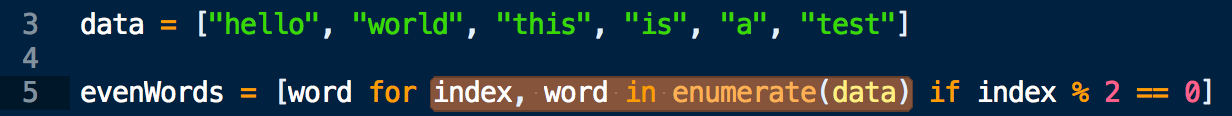
\includegraphics[width=0.95\columnwidth]{figures/highlight.png} 

\end{itemize}

Note that all these limitations of written tutorials are not specific to
Google Docs; related tools likely face similar issues.

\rev{Although we did not directly compare Torta to screencast videos for
this study, several creators mentioned the similarities between Torta
and screencast recording. For instance, S5 said, \emph{``This [Torta]
isn't any different from recording a screencast and I can also do
editing, annotation and validation."} And S2 mentioned, \emph{``I think I
would use this over recording a screencast despite the additional
processing time since the editor allows easier basic editing, like
dropping steps, which is easier than using a full video editor."}}

Subjects also conveyed perceived shortcomings of Torta's creation
workflow: It took some a while to get used to Torta segmenting videos
based on OS events such as GUI window switches, so they had to learn to
finish a full sentence of narration before switching in order to avoid
awkward audio cuts. They wanted to have more diverse format choices
than the step-by-step GUI-window-delimited structure that Torta imposes.
They also felt written tutorials were more flexible and less constraining,
though they take much more work to make.

Finally, \tab{tab:creator-study} shows that 9 out of 10 subjects created tutorials faster using Torta than
Google Docs.
For the five who used Torta first, they took around 1.1 times longer to
create the GDocs version (the harmonic mean of their time differences);
for the five who used GDocs first, they took an average of 2 times
longer in GDocs. This speed difference is likely due to them needing to spend
time planning out their tutorial's structure during their first attempt,
regardless of tool. \rev{This phenomenon likely resulted in a significant learning
effect since by the time they tried the second condition, they already
knew exactly what tutorial they wanted to create.} However, even when using
Torta first, subjects still
found it to be slightly faster. But we do not want to overemphasize these
timing numbers because the primary design goal of Torta was not to optimize
for tutorial creation speed.


\subsection{Tutorial Consumer \rev{Pilot Study}}

Although in the prior study we had creators self-assess the quality of their own Torta and
GDocs tutorials, we also wanted to get an assessment from the actual
target audience: students. Thus, we ran a \rev{follow-up pilot study} where students
followed the tutorials created by the TAs in the prior study and
compared their perceptions of Torta vs.\ GDocs from their perspectives
as tutorial consumers.


\emph{\textbf{Procedure}}: We recruited 6 undergraduate computer science
students each for a one-hour lab study. We had 3 subjects try to follow
a Torta-generated tutorial; then we showed them the Google Docs version
of the \emph{same} tutorial and had them compare and contrast the two
formats. We had the other 3 subjects try to follow a Google Docs
tutorial, and then had them compare it to its Torta counterpart. We did
not have each subject try to follow both tutorials since they would already
know how to perform the task after following the first one.

For this study, we picked the Node.js web programming tutorial created by
S2 since it was the most complex one. However, two subjects did
not have enough technical background to understand it, so instead we
gave them the singly-linked list tutorial created by S7 (one used
Torta, one used GDocs).


\emph{\textbf{Results}}: All 6 subjects successfully completed the
tutorial tasks in their given format. Both sets of 3 subjects (i.e.,
those who tried to follow the Torta tutorial then saw the Google Docs
version, and vice versa) preferred consuming Torta tutorials over Google
Docs for a variety of reasons, including:

%in \todo{15--18 minutes}; there were no major noticeable differences in
%completion times between Torta and Google Docs.


\begin{itemize}\itemsep0pt

\item \emph{Torta tutorials were better-structured}: Once subjects got
used to Torta's structure, they appreciated its predictability and could
skip over parts that did not interest them. In contrast, GDocs does not
impose any structure, so tutorials created within it felt more uneven in
pace. Subjects also commented that the consistency in Torta's format
would be good for a series of related tutorials across an entire course.

\item \emph{Torta tutorials more information-dense}: Most subjects
commented that Torta tutorials were more information-dense than GDocs
since they were narrated by voice and included automatically-traced
filesystem and command info. The GDocs versions could not include many
details due to lack of time for creators to write out everything
explicitly.

\item \emph{GUI apps better explained with mini-videos}: All subjects
felt that video was a much better way to demonstrate GUI applications
such as Postman rather than seeing a series of screenshots in GDocs.
They also appreciated each video being short and focused on only one
window.

\item \emph{Torta provides context behind file diffs}: When using GDocs
to create tutorials involving code, most creators ended up simply
pasting the new bits of code written in each step into the doc without
adequate surrounding context. Thus, subjects were confused about where
those pieces of code were supposed to be placed. In contrast, Torta
automatically generates file diffs and shows the original file contents
along with mini-videos to give students the proper context.

\item \emph{Torta's Validate and Run buttons were popular}: All
Torta-using subjects tried the Validate and Run buttons and commented that they seemed very
useful. They liked using Validate to avoid minor errors
compounding in later steps.

%\item \emph{Torta's collapsable steps were useful}: Several subjects
%used the collapse button next to steps and sub-steps to mark those
%parts as ``done" when they were following the tutorial so that they
%could keep track of their place.


\end{itemize}

However, one student (who had the most web dev experience) preferred
skimming a well-written GDocs tutorial rather than having to play the
Torta mini-videos and listen to audio narration at each step. Torta also
lets creators write HTML annotations for each step, but due to our user
study's short time limit, creators did not write much text in their
Torta tutorials.

\rev{Finally, although we did not directly compare Torta to
raw screencast videos for this study, several subjects
implicitly compared Torta with their prior experiences of watching
screencasts. For instance,
S11 said, \emph{``A lot of times when I'm watching coding videos on
YouTube, I wish I would have had a way to copy code and commands. This
[Torta] makes that way easier."}
%
S13 said: \emph{``I think cropping videos to the frontmost window is
great since it narrows focus to just that window. Many screencasts I
watch record the entire screen."}
%
S13 also mentioned: \emph{``I liked Torta breaking the video into steps.
On YouTube, video descriptions sometimes have links to different parts
of the video but using this [Torta] is much easier because I see the
parts of the video already split up."} }


\section{Discussion of Design Space and Limitations}
%\section{Discussion: Design, Limitations, \& Future Work}

Torta carves out a new point in the design space of
tools for generating step-by-step records of app actions
(\fig{fig:design-space}).
%
In contrast to prior systems that operate within a single application,
Torta is designed to be as application-agnostic as possible so that it
can work across arbitrary desktop applications. This design decision
means \textbf{\emph{giving up granularity for generality}}: Torta cannot perform
fine-grained domain-specific tracking within any particular application, but
rather operates at the level of GUI windows, shell commands, system
calls, and filesystem mutations. One future way to bridge this gap is to
implement a plug-in system similar to Burrito's~\cite{GuoBurrito2012} where users write
application-specific tracers to hook into Torta.


On the spectrum of manual to automated running of steps, Torta lies
mostly at the manual end. Its primary goal is to generate mixed-media
tutorials for people to consume by manually following the steps and
customizing based on their needs. In contrast, fully-automated scripting
engines serve a different purpose than tutorials: Their goal is to
automate a set of repetitive actions, \emph{not} to show people how to
manually perform those actions with accompanying pedagogical context. In sum,
Torta's output should primarily be thought of as a \emph{rich form of
documentation} to help people figure out how to perform tasks for themselves,
not as a fully-automated script.


Torta is situated at a point in the design space \rev{that makes it
well-suited for a range of filesystem-modifying and
command-line-heavy} software tasks.
%
%, so they are well-suited for Torta.
%
Even though our original motivation was full-stack
web development, Torta is also useful for other complex software
development tasks involving more than simply an IDE. For instance,
game programming tutorials use an IDE, a 3D level editor, various
multimedia editors for assets, and project management tools all tied
together by command-line scripts. Low-level systems programming
tutorials involve a mix of command-line and GUI tools for introspection,
debugging, and performance profiling. Sysadmin (system administration)
and DevOps tutorials touch many corners of the operating system at once.
Data science tutorials combine multiple programming languages with
GUI-based data acquisition/wrangling tools. Finally, scientific
researchers hack up ad-hoc workflows that span multiple scripting
languages, scientific libraries, and legacy research
tools~\cite{GuoPhD2012}, so they can use Torta to generate documentation
that can help colleagues reproduce and build upon their computational
experiments.
%
\rev{However, Torta is less well-suited for information-foraging-heavy
computing tasks such as scholarly research and CSCW-types of
communication workflows, since those involve fewer filesystem
modifications and shell commands. For those kinds of tasks, Torta simply acts
like a screencast recorder with window-based segmentation.}


\begin{figure}
%\vspace{16em}

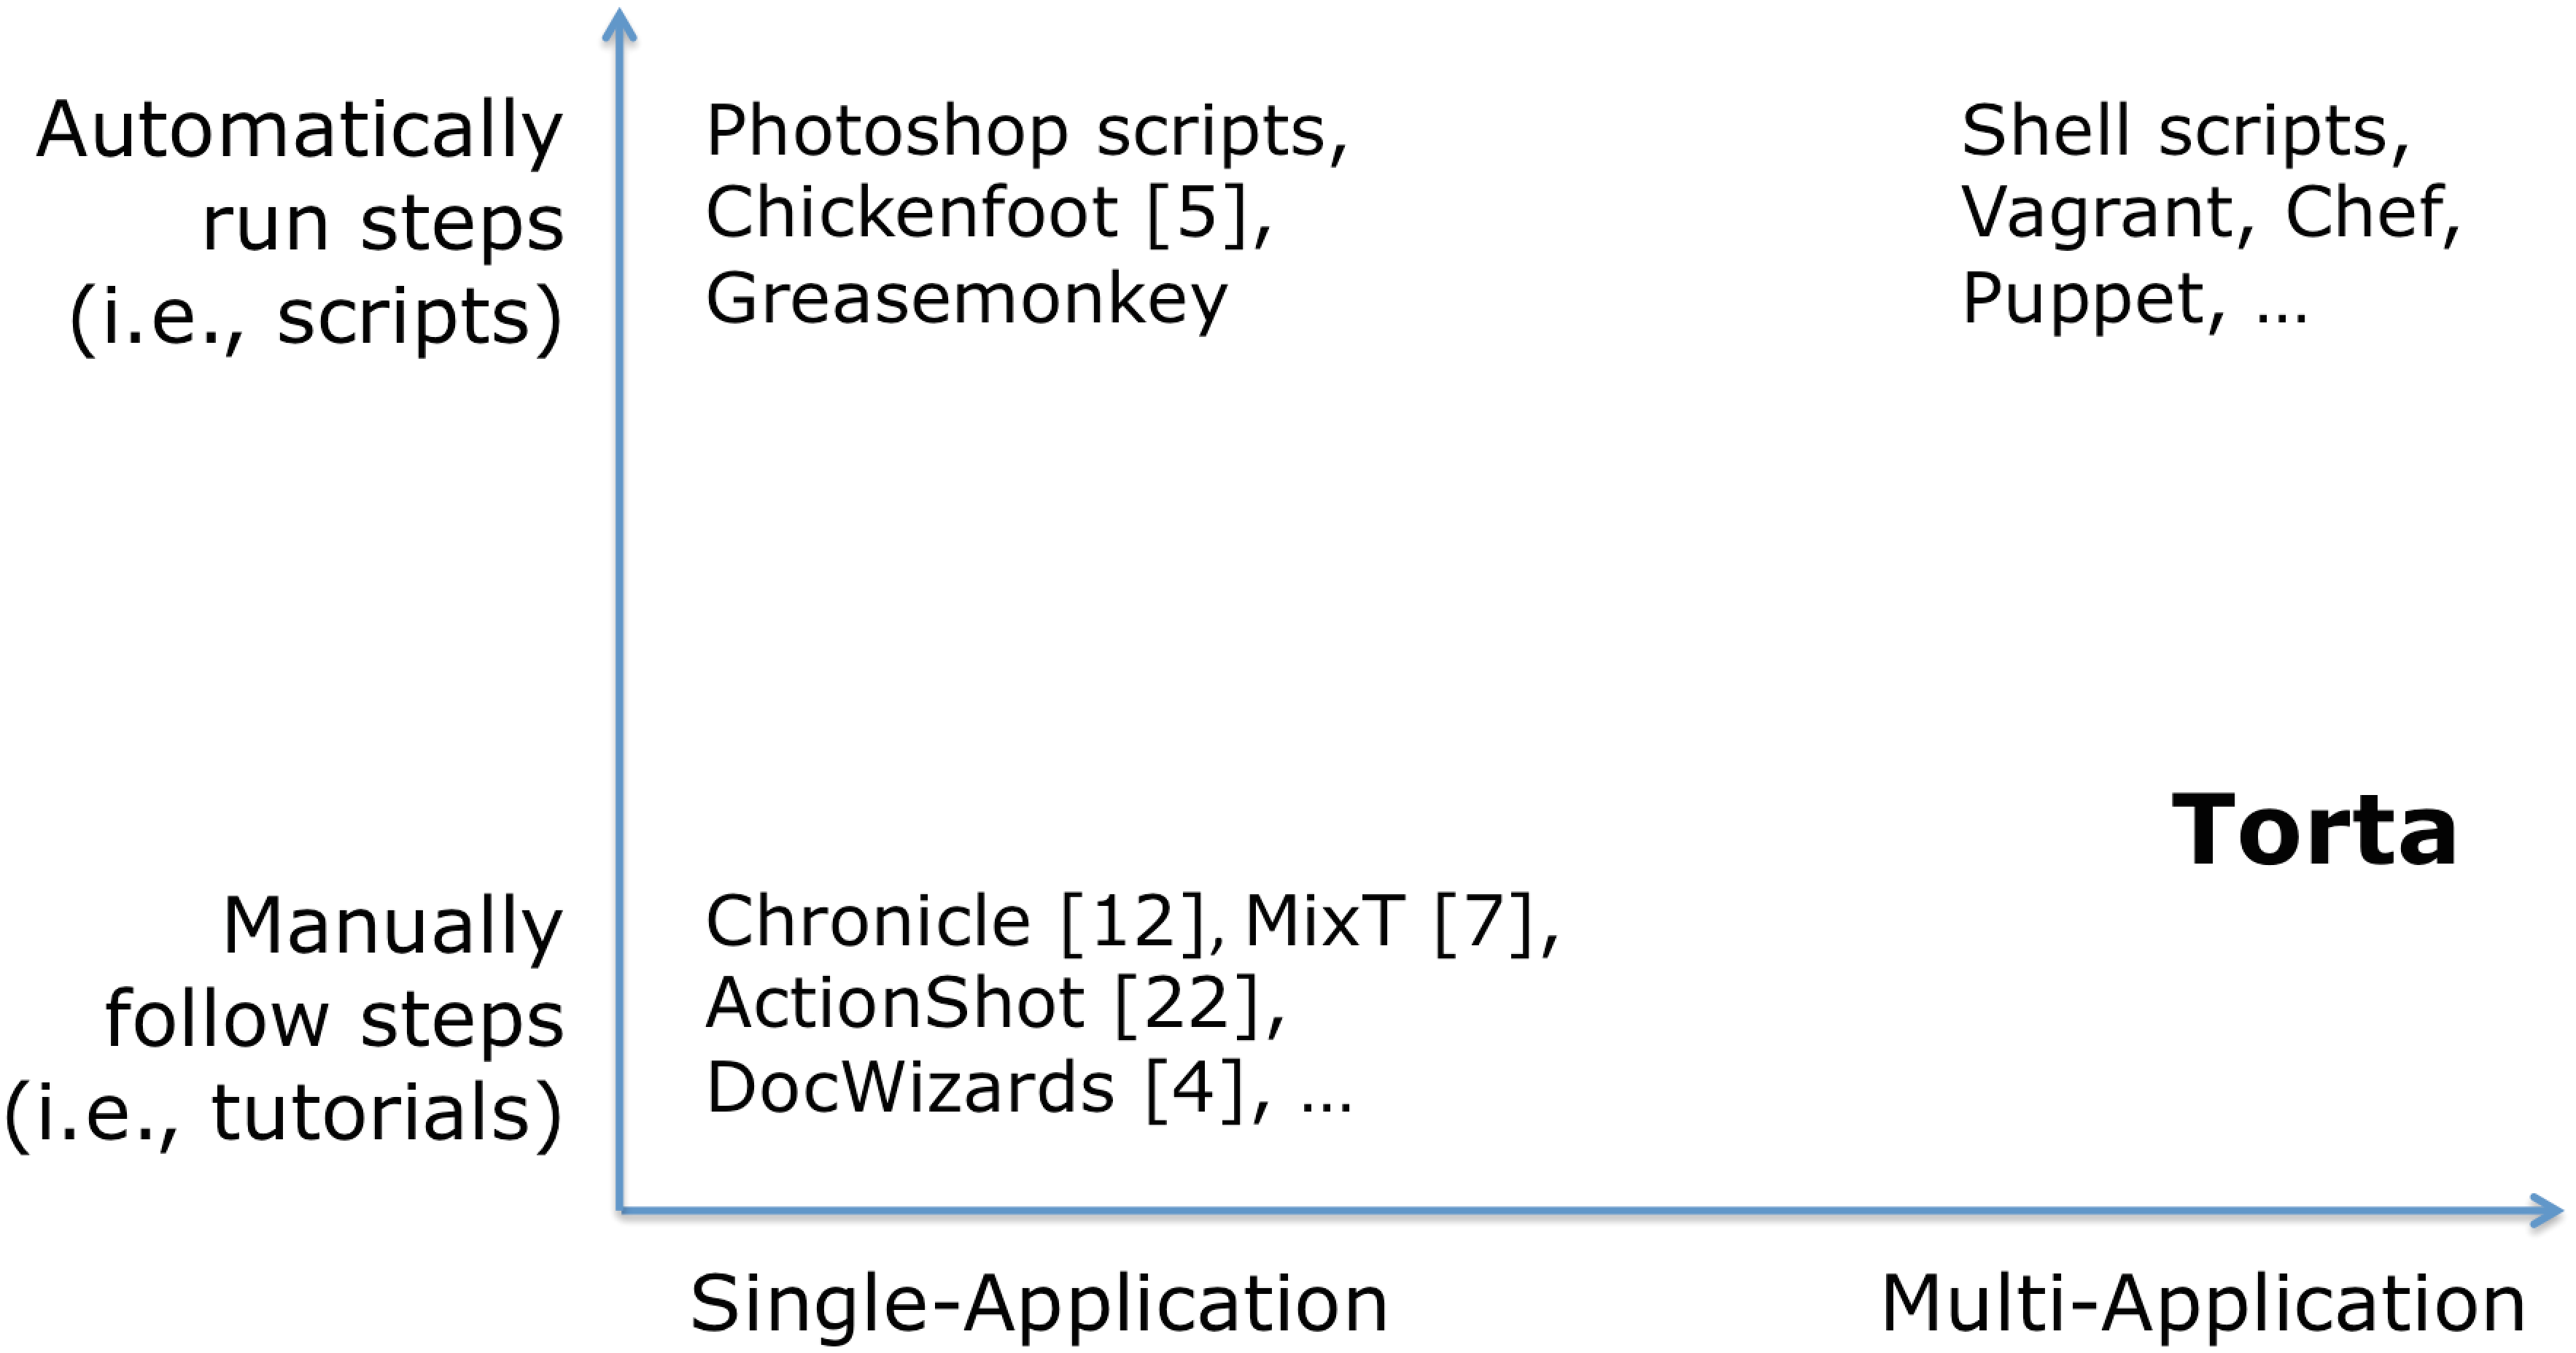
\includegraphics[width=\columnwidth]{figures/torta/design-space.png}

\nocite{Bolin2005} % cite Chickenfoot in the figure
\caption{The design space of tools for generating step-by-step records
of application actions, ranging from those that automatic run (i.e.,
scripts) to those meant for users to manually follow their steps (i.e.,
tutorials).}

\vspace{-0.5em} % stent
\label{fig:design-space}
\end{figure}


One of Torta's current limitations is that it supports recording and
editing only one user demonstration at a time. A future version of the
editor could support intelligent merging of multiple demonstrations
based on OS activity traces. Another limitation is that Torta does not
try to generalize the tutorial's contents: All recorded steps are
specific to the creator's single demonstration. Thus, it is up to the
creator to manually describe how each step could potentially be
generalized or customized by consumers. Again, a more intelligent editor
could take multiple demonstrations and semi-automatically infer possible
generalizations to make tutorials more robust.

Finally, even though automatically running certain steps can be
convenient, we have purposely not designed the Torta viewer as an
fully-automated tutorial runner. Differences between users' OS
setups and properties of specific applications make it impossible to
automatically run all steps with full accuracy.
Thus,
we still intend for users to manually follow tutorial steps and
only use automatic running as a supplement.


\section{Conclusion}

We presented Torta, an end-to-end system for recording, editing, and
consuming \rev{mixed-media tutorials that span multiple GUI and
command-line applications. The core technical insight that underpins
Torta is that the operating system already keeps track of vital
filesystem and process-level metadata necessary for segmenting tutorial
steps}. Thus, combining operating-system-wide activity tracing with
screencast video recording makes it possible to quickly create complex
GUI and command-line app tutorials by demonstration. \rev{Torta's
application-agnostic design} makes it well-suited for creating
tutorials in domains such as software development, data science, system
administration, and computational research.
%
\rev{We hope that it will inspire the design of future tutorial systems
that bridge the gap between video- and text-based formats.}





\bibliographystyle{SIGCHI-Reference-Format}
\bibliography{references}

\end{document}


\bibliographystyle{alpha}
\bibliography{references}

\end{document}